%%% -*- Mode: LaTeX; indent-tabs-mode: nil -*-
%%%
%%% Copyright (c) 2004, Oliver Markovic <entrox@entrox.org> 
%%%   All rights reserved. 
%%%
%%% Redistribution and use in source and binary forms, with or without
%%% modification, are permitted provided that the following conditions are met:
%%%
%%%  o Redistributions of source code must retain the above copyright notice,
%%%    this list of conditions and the following disclaimer. 
%%%  o Redistributions in binary form must reproduce the above copyright
%%%    notice, this list of conditions and the following disclaimer in the
%%%    documentation and/or other materials provided with the distribution. 
%%%  o Neither the name of the author nor the names of the contributors may be
%%%    used to endorse or promote products derived from this software without
%%%    specific prior written permission. 
%%%
%%% THIS SOFTWARE IS PROVIDED BY THE COPYRIGHT HOLDERS AND CONTRIBUTORS "AS IS"
%%% AND ANY EXPRESS OR IMPLIED WARRANTIES, INCLUDING, BUT NOT LIMITED TO, THE
%%% IMPLIED WARRANTIES OF MERCHANTABILITY AND FITNESS FOR A PARTICULAR PURPOSE
%%% ARE DISCLAIMED.  IN NO EVENT SHALL THE COPYRIGHT OWNER OR CONTRIBUTORS BE
%%% LIABLE FOR ANY DIRECT, INDIRECT, INCIDENTAL, SPECIAL, EXEMPLARY, OR
%%% CONSEQUENTIAL DAMAGES (INCLUDING, BUT NOT LIMITED TO, PROCUREMENT OF
%%% SUBSTITUTE GOODS OR SERVICES; LOSS OF USE, DATA, OR PROFITS; OR BUSINESS
%%% INTERRUPTION) HOWEVER CAUSED AND ON ANY THEORY OF LIABILITY, WHETHER IN
%%% CONTRACT, STRICT LIABILITY, OR TORT (INCLUDING NEGLIGENCE OR OTHERWISE)
%%% ARISING IN ANY WAY OUT OF THE USE OF THIS SOFTWARE, EVEN IF ADVISED OF THE
%%% POSSIBILITY OF SUCH DAMAGE.

\chapter{Controller}

\section{Generelles Konzept zur Businesslogik}

\begin{figure}[!h]
\begin{center}
  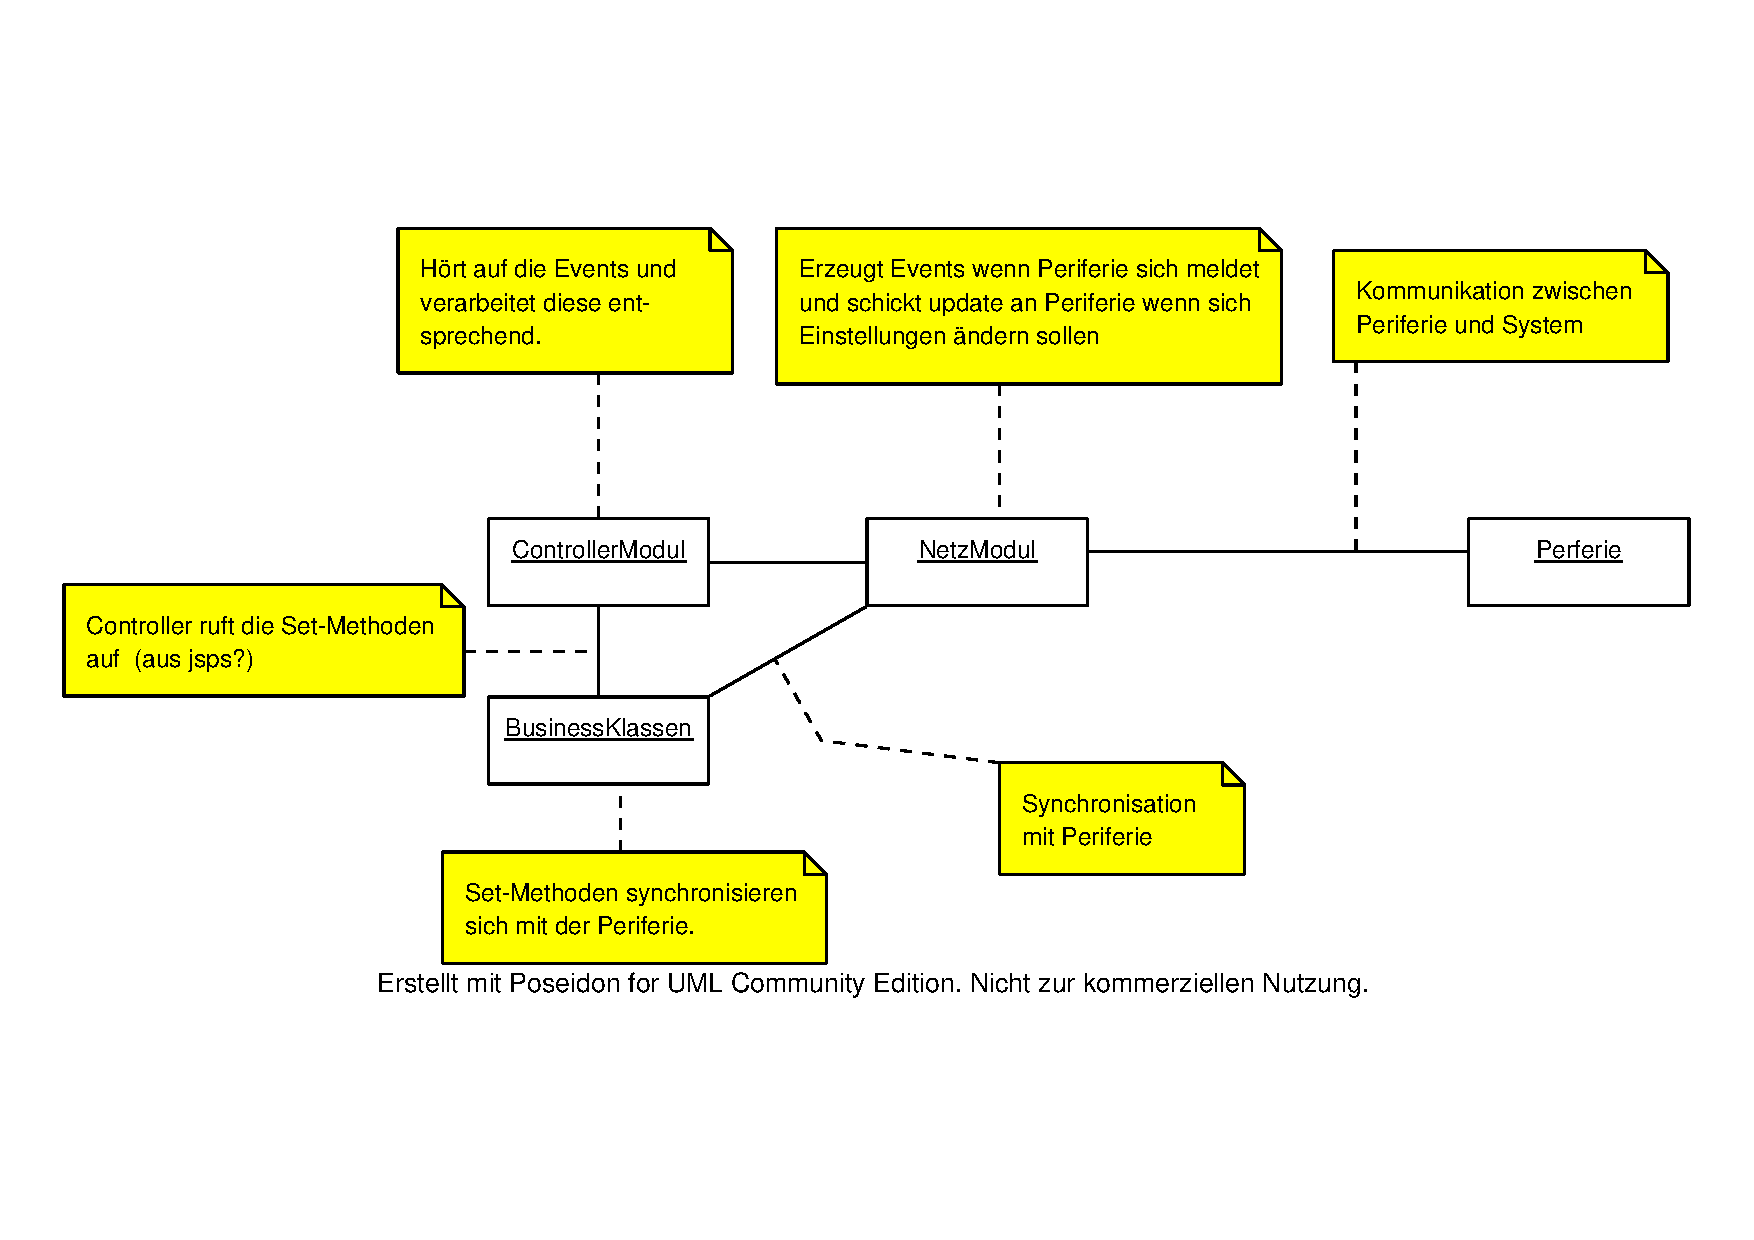
\includegraphics[width=360pt]{logischer_zusammenhang_controller.pdf}
  \caption{Zusammenhang der Komponenten}
\end{center}
\vspace*{-6mm}
\end{figure}
\newpage
\section{Beschreibung der Logik}
Im Folgenden wird der Entwurf der grundlegenden Szenarien beschrieben.\\
\begin{itemize}
\item Szenario 1: Das System wird gestartet.
\item Szenario 2: Ein Benutzer betritt den Raum.
\item Szenario 3: Ein Benutzer �ndert seine Profileinstellungen.
\end{itemize}

\subsection{Klassen und Methodenbeschreibung}

\begin{figure}[!h]
\begin{center}
  \includegraphics[width=360pt]{Klassen_Controller.pdf}
  \caption{Klassen und Methoden f�r die Businesslogic}
\end{center}
\vspace*{-6mm}
\end{figure}

\subsubsection{BusinessKlassen}

\textbf{UserLogin logIn()}
\begin{itemize}
	\item Meldet den Benutzer am Betriebsystem an.
	\item Setzt den Benutzer auf eingeloggt.
	\item L�dt das Defaultprofil des Benutzers\\
\end{itemize}

\textbf{UserLogin logOut()}
\begin{itemize}
	\item Meldet den Benutzer vom Betriebsystem ab.
	\item Setzt den Benutzer auf nicht eingeloggt.
	\item Setzt alle Komponenten auf ihre Defaulteinstellung.\\
\end{itemize}

\textbf{SmartRoomComponent static getComponent(String description)}
Der Wert \textit{description} enth�llt die id der Komponente.
\begin{itemize}
	\item Falls die Komponenten-Instanz mit der id schon existiert (im Speicher), liefert sie zur�ck.
	\item Falls die Komponenten-Instanz mit der id noch nicht existiert, wird die Komponenten-Instanz anhand der description erzeugt.\\
\end{itemize}

\textbf{SmartRoomComponent remove()}
\begin{itemize}
	\item Entfernt alle Eintr�ge aus den Benutzerprofilen, die zu dieser Komponente geh�ren .\\
\end{itemize}

\textbf{SmartRoomComponent setIsActive(Boolean isActive)}
\begin{itemize}
	\item Setzt die Komponenten-Instanz auf aktiv / inaktiv.
	\item Nur aktive Komponenten werden angezeigt.\\
\end{itemize}

\textbf{SmartRoomProfil load()}
\begin{itemize}
	\item Setzt alle zum Profil geh�rigen Properties. 
	\item Das Setzen der Properties bewirkt deren synchronisation mit der Periferie.\\
\end{itemize}

\textbf{ComponentProperie setValue(ComponentProperieValue value)}
\begin{itemize}
	\item Wenn Benutzer eingeloggt ist, Synchronisation mit der Periferie.\\
\end{itemize}


\textbf{NetzContoller StandardEvents}
\begin{itemize}
	\item signalUserIn (OPS) - Ein Benutzer hat den Raum betreten. 
	\item signalUserOut (OPS) - Ein Benutzer hat den Raum verlassen. 
	\item signalPropertieChange (MediaCenter) - Eine Properie wurde gesetzt/ver�ndert.\\
\end{itemize}

\textbf{NetzContoller init()}
\begin{itemize}
	\item sendet broadcast, woraufhin sich alle Componenten melden sollen.\\
\end{itemize}

\textbf{NetzContoller signal(Event event)}
\begin{itemize}
	\item l�st ein Event aus.\\
\end{itemize}


\textbf{UserEventListener handleEvent()}
\begin{tabbing}
xxxx\=xxxxxxxxx \kill
Auf: "`TagID rein"'\\
\>-> Hohl Benutzer; Benutzer.logIn();\\
Auf: "`Benutzer rein"'\\
\>-> Benutzer.logIn();\\
Auf: "`Benutzer raus"'\\
\>-> Benutzer.logOut();\\
Auf "`TagID raus"'\\
\>-> Hohl Benutzer; Benutzer.logOut();\\
\end{tabbing}


\textbf{MarsComponentListener initComponents()}
\begin{itemize}
	\item Initialisiert das Netz\\
\end{itemize}

\textbf{MarsComponentListener handleEvent()}
\begin{tabbing}
xxxx\=xxx\=xxxxxx \kill
1. Auf: "`Hallo, ich bin da"'\\
		\>-> ist Componente schon initialisiert und ist sie aktuell.\\
    \>\> true -> nix\\
    \>\> false -> hohle Beschreibung; initialisiere Componente mit Beschreibung;\\
2. Auf: "`Tsch�ss"'\\
    \>-> ist Componente bekannt:\\
    \>\> true -> Componente.setIsActive(false);\\
\end{tabbing}

\textbf{MarsComponentListener setProperie(String id, PropertyValue value)}
\begin{itemize}
	\item L�dt Property mit dazugeh�riger ID
	\item Setzt das Value der Propery mit Value
\end{itemize}

\subsection{Szenario 1 - Starten des Systems}
Das Netzmodul sendet einen Broadcast ins Netz, woraufhin sich die einzelnen Komponenten melden.
Das Netzmodul signalisiert jede sich meldende Komponente an den Komponenten-Listener. Dieser speichert die Beschreibungen zur Komponente in der Datenbank.

\subsection{Szenario 1 - Ein Benutzer betritt der Raum}
Das OPS signalisiert "`BenutzerX hat den Raum betreten"'. Der UserController meldet den Benutzer am Betriebsystem an und l�dt dessen Defaultprofil.

\subsection{Szenario 3: Ein Benutzer �ndert seine Profileinstellungen.}
Ein Benutzer �ndert �ber das MediaCenter seine Einstellungen. Das MediaCenter signalisiert: PropertyX hat sich auf ValueX ge�ndert. Der ComponentenListener setzt die entsprechende Property im Speicher auf das gegebene Value. Durch den Setzvorgang wird die Periferie synchronisiert.
